% Nome do capítulo
\chapter{Deep Learning}
\label{cap2_redes_neurais}

%TODO Definição de rede neural com fórmula ax+b
% Texto do capítulo
The first learning algorithms were created with a vague inspiration in the functioning of the human brain.
These algorithms were then called Artificial Neural Networks (\acused{ANN}\ac{ANN}).
Adding layers to \acused{ANNs}\ac{ANNs} has given rise to multilayer networks, called Deep Neural Networks (\acused{DNN}\ac{DNN}). 
The term deep learning arose from the use of these networks \cite[Ch. 6]{Goodfellow2016} \cite{ShalevShwartz:2014:UML:2621980}.

This chapter presents the main concepts related to artificial neural networks, especially those where there is deep learning.
The organization of the chapter was based on \citeonline{Goodfellow2016} e \citeonline{ShalevShwartz:2014:UML:2621980}. 
It is organized as follows: Section \ref{cap2_nn_feedforward} contains feedforward neural networks; Section \ref{cap2_regulariz_deep_learning} details regularization techniques; Section \ref{cap2_met_treinamento} describes training methods; and, finally, Section \ref{cap2_nn_convolucionais} defines convolutional neural networks, convolution, transposed convolution and pooling operarions.
%-----------------------------------------------

%-----------------------------------------------
% - REDES NEURAIS FEEDFOWARDING	
\section{Feedforward Neural Networks}
\label{cap2_nn_feedforward}

Feedforward neural networks, also know as Multilayer Perceptron (\acused{MLP}\ac{MLP}) have neurons grouped in layers.
The information moves in a single direction from an input $x$ to an output $y$ and can go through intermediate steps \cite[Ch. 6]{Goodfellow2016}.

Feedforward neural networks are the basis for other types of more complex networks, such as convolutional neural networks \cite[Ch. 6]{Goodfellow2016}. 
Formally, they are described as an acyclic graph $G=(V,E)$, where the nodes correspond to the neurons and the edges correspond to the relationship between neurons, with an associated weights $w_{ij}$, between two nodes $i$ and $j$ \cite{ShalevShwartz:2014:UML:2621980}.

Feedforward neural networks receives an input vector $X$, called domain set, and are expect to produce a target vector $Y$, called label set, that correspond to correct answers to the problem. 
The network is trained, to adjust it weights, and to produces an output $\hat{Y}$, that are compared to the label set $Y$.
The inaccuracies between the output $\hat{Y}$ and the target value $Y$ is called error $E$ \cite{Marsland:2014} \cite{ShalevShwartz:2014:UML:2621980}.

In the network, each neuron can be defined as a scalar function $f(x): \mathbb{R} \rightarrow \mathbb{R}$ and chain neuron compositions can be performed in the form of $f(x) = f^{(3)} (f^{(2)} (f^{(1)} (x)))$ . 
The layer $f^{(1)}$ it's called the first layer, $f^{(2)}$ and $f^{(3)}$ are the second and the third ones, respectively, and, if $f^{(2)}$ is not an output layer, it is called the middle or hidden layer.
Finally, the number of network layers provides the depth of the model \cite{ShalevShwartz:2014:UML:2621980} \cite[Ch. 6]{Goodfellow2016}.

%-----------------------------------------------
%SUB - APREND. BASEADO GRADIENTE
\subsection{Neural Network Learning}
\label{cap2_nn_learning}

Neural networks are generally trained with iterative gradient-based methods to minimize a loss function.
This commonly uses the principle of maximum likelihood, using, for example, a negative \textit{log} probability function \cite{Goodfellow2016}. 

In the network output layers, various types of operations are used, such as \textit{max} functions, \textit{sigmoid}, \textit{softmax}, \ac{ReLU}, among others \cite[Ch. 8]{Goodfellow2016}. 
These functions can also be used for activating the intermediate layers.

%-----------------------------------------------
%SUB - BACKPROPAGATION E SGD
\subsection{Back-propagation and Stochastic Gradient Descent}
\label{cap2_nn_feed_backpropag}

The \textit{feedforward} network uses the input-to-output value propagation method known as forward propagation. 
The \textit{back-propagation} method allows partial derivatives losses to return from the final layers to the initial network layers \cite[Ch. 8]{Goodfellow2016} \cite{Rumelhart1988}. 

The back-propagation method computes only the gradient between the desired value and the loss, while other algorithms, such as \ac{SGD}, use the gradient value to update the weights.
The procedure allows node weights to be continuously adjusted so that the model can minimize loss by learning from attempt and adjustment \cite[Ch. 8]{Goodfellow2016} \cite{Rumelhart1988}.

\ac{SGD} is an iterative method based on the gradient method. 
This takes the negative direction of the gradient, corresponding to the maximum slope, in order to find a local minimum.
In the \ac{SGD} method, instead of taking the maximum negative direction of the gradient, a random direction of a set of gradients is taken, requiring only that the expected value be equal to the gradient direction value \cite[Ch. 8]{Goodfellow2016}. 

%TODO Revisar citações
Although it seems counterintuitive for the algorithm to take a random direction rather than the minimum direction, this step prevents the \ac{SGD} from stalling at a local minimum point and is more likely to reach or approach the global maximum of the function \cite{Kiwiel2001ConvergenceAE}. 
Like the gradient method, the \ac{SGD} uses a parameter corresponding to the step size in the minimum direction, called \ac{LR}, which indicates how far the algorithm will move toward the minimum.
This rate enables the algorithm to move toward the minimum faster, but less accurately, or slower, with greater accuracy.
%-----------------------------------------------

%-----------------------------------------------
% - REGULARIZAÇÃO DEEP LEARNING
\section{Deep Learning Regularization}
\label{cap2_regulariz_deep_learning}

Strategies to decrease error in the neural network test step, even if they increase errors in training steps, are called regularization.
In neural networks, penalty mechanisms may be adopted to regulate cost functions.
These mechanisms add a penalty parameter $\Omega(\theta)$ to penalize weights whose values do not match the desired result in the objective function $J$ \cite[Ch. 7]{Goodfellow2016}.

\begin{comment}
A regularização $L^2$ é um tipo de regularização conhecido como decaimento de pesos, que consiste na adição de um termo de regularização $\Omega$ na função objetivo, conforme Equação \ref{eq:cap2_regularizacao_l2}:

\begin{equation}
 \Omega (\theta) = \frac{1}{2} {\parallel{\omega}\parallel}^2_2
 \label{eq:cap2_regularizacao_l2}
\end{equation}

A regularização $L^2$ penaliza vetores de pesos com valores altos e prefere vetores com pesos difusos, levando a rede neural a utilizar todos os seus neurônios, ao invés de somente aqueles que tiveram bons resultados em uma etapa do treinamento \cite{Goodfellow2016}.

%TODO: revisar referências
A regularização $L^1$ é um tipo de regularização que leva o vetor de peso a ter valores próximos de zero durante a etapa de treinamento. 
Utiliza apenas um subconjunto distribuído no vetor de pesos (esparso) das entradas mais importantes, diminuindo a susceptibilidade às entradas que contém ruídos \cite{Goodfellow2016}. 
É definido para um modelo de parâmetro $\omega$ segundo a Equação \ref{eq:cap2_regularizacao_l1}.

\begin{equation}
 \Omega (\theta) = \frac{1}{2} {\parallel{\omega}\parallel}_1 = \sum_{i}^{\infty} |{\omega}_i|
 \label{eq:cap2_regularizacao_l1}
\end{equation}
\end{comment}

%-----------------------------------------------
%SUB - DATA AUGMENTATION
\subsection{\textit{Data set augmentation}}
\label{cap2_data_augmentation}

Data set augmentation consists of a set of transformations applied to the database to increase the number of records for training.
This procedure seeks to increase the accuracy and robustness of the classifiers. \cite{ADAPT_DT_AUGM:2016:7533048}. 
The measure is mainly applied to databases with few records, whose training models do not generalize well \cite{Perez:2017:EFF_DT_AUGM}.

Data set augmentation can act as a type of regularizer avoiding overfitting and increasing performance in problems where class imbalance occurs \cite{Wong:2016:UNDERST_DT_AUGM}, such as in edge detection problems, where the number of edge pixels is significantly less than the number of non-edge ones.

%-----------------------------------------------
%SUB - BAGGING E METODOS ENSEMBLE
\subsection{Bagging and Ensemble}
\label{cap2_bagging_ensemble}

Bagging is short for bootstrap aggregating, a technique for reducing generalization error by creating multiple versions of a predictor and using them to create an aggregate predictor \cite{Breiman1996}. 
Prediction values are used for a single numerical result based on individual votes.
The techniques that use this strategy are called ensemble methods \cite{Breiman1996} \cite[Ch. 7]{Goodfellow2016}.

The idea behind ensemble methods is that each predictor will make one type of error and that multiple predictors will tend to miss less when combined \cite{Goodfellow2016}, since the errors of each will be suppressed by the successes of the others.
For this it is necessary that the predictors produce different errors covering all the possible space, so that the error of one predictor is not ratified by the others.

%-----------------------------------------------
%SUB - DROPOUT
\subsection{\textit{Dropout}}
\label{cap2_dropout}

Dropout is a regularization method that seeks to train the entire set of subnets in a neural network.
Considering a network as a set of subnets that perform ensemble, it is possible to eliminate non-output unit values by multiplying their value by zero.
This technique aims to get the whole network trained, not just parts that they learned at first \cite[Ch. 7]{Goodfellow2016}.

The dropout mechanism is able to avoid overfitting the network, where the network learns training data, but cannot generalize to a test suite. 
The amount of neurons that will be zeroed in the dropout layers is given by a parameter set before training, which indicates how much the network will ignore from its prior learning to learn new information \cite{Srivastava2014Dropout}.

%-----------------------------------------------
%SUB - BATCH NORMALIZATION
\subsection{\textit{Batch Normalization}}
\label{cap2_batch_normalization}

Batch Normalization is a method for regularization, aiming to keep each neural network layer with zero mean and unit variances,  increasing the convergence speed. 
The method consists in decreasing the change in internal covariate shift, corresponding to the changes in the distribution of network activations.
For this, the inputs of each layer are normalized for every training mini-batch.
The method allows, in several scenarios, to increase the learning rates, to initialize parameters with less care and to remove other regularization techniques. \cite{Ioffe2015:pmlrv37}.
%-----------------------------------------------

%-----------------------------------------------
% - MÉTODOS DE TREINAMENTO
\section{Training Methods}
\label{cap2_met_treinamento}

Training methods seeks to find a set of parameters that can minimize the cost function, producing the lowest possible loss \cite[Ch. 7]{Goodfellow2016}.

%-----------------------------------------------
%SUB - Minimização de risco empírico
\subsection{Empirical Risk Minimization}
\label{cap2_minimiz_risco}

Minimizing empirical risk is a statistical process that seeks to minimize expected loss in training.
The average loss is minimized in the hope that decreasing this error may also decrease the actual risk of loss in the test set, unknown during the training step.
Risk minimization, however, is subject to the overtraining effect, where the error decreases in the training stage but increases in the testing stage.
In this scenario, the network learns training data, rather than generalizing its knowledge \cite[Ch. 7]{Goodfellow2016}.

%-----------------------------------------------
%SUB - ESTRATEGIAS INCIALIZACAO
\subsection{Parameter Initialization Strategies}
\label{cap2_inic_parametros}

Gradient methods are sensitive to initialization of parameters used in neural networks.
Poor initialization of values may not guarantee the convergence of non-convex functions and some strategies used correspond to simple heuristics, which seek to establish common characteristics at initialization \cite[Ch. 7]{Goodfellow2016}.

Parameter initialization in multi-tier architectures, especially using random values, can cause intermediate layers to be saturated, so that the initialized values are not harnessed in those layers.
After multiple layers, the average value tends to zero, as well as the standard deviation, making the learning rate small \cite{Glorot2010a:PMLR}.

%-----------------------------------------------
%SUB - TRANSFER LEARNING
\subsection{Transfer Learning}
\label{cap2_transfer_learning}

Transfer learning is a learning technique in which knowledge gained from solving one problem is transferred to another. 
A neural network developed for one problem is adapted and applied to a different but related problem.
This technique has been performed for many years and prevents it from being ``reinvented the wheel'' as knowledge begins at a later stage in the training process. \cite{Pratt:1992:NIPS1992_641} \cite{Weiss:2016:JOURN_BIG_DATA}.

%-----------------------------------------------
%-----------------------------------------------
%-----------------------------------------------
% - REDES NEURAIS CONVOLUCIONAIS
\section{Convolutional Neural Networks}
\label{cap2_nn_convolucionais}

Convolutional networks are a specialized type of neural networks that use a mathematical operation called convolution in at least one of its layers \cite[Ch. 9]{Goodfellow2016}.

%-----------------------------------------------
%SUB - OPERAÇÃO CONVOLUÇÃO
\subsection{Convolution Operation}
\label{cap2_convolucao}

Convolution is a linear operator for two functions $f$ and $g$, resulting in a third value $s$ that measures the sum of the product over the region implied by the superposition of $g$, when shifted over a function $f$ \cite{ConvolutionMathWorld:2018}. 
The concept of convolution is linked to overlay integration and can be understood as the way a system operates over an input signal. \cite[Ch.~6]{Smith:1997:SEG:281875}.

The notation of convolution operation $s$ between two functions $f$ and $g$ is given by the Equation \ref{eq:cap2_convolucao_def} \cite[Ch. 9]{Goodfellow2016}.

\begin{equation}
 s(t) = (f * g)(t)
 \label{eq:cap2_convolucao_def}
\end{equation}

A continuous convolution in an infinite interval $[{-}\infty, \infty]$, corresponds to the integral of the product of one function by an offset and inverted copy of the other, whose notation is given by Equation \ref{eq:cap2_convolucao_cont} \cite{ConvolutionMathWorld:2018}.

\begin{equation}
 (f * g)(t) = s(t) = \int_{{-}\infty}^{\infty} f(u) \cdot g(t-u)du
 \label{eq:cap2_convolucao_cont}
\end{equation}

A discrete version of continuous convolution in a interval $[{-}\infty, \infty]$, is given by the Equation \ref{eq:cap2_convolucao_disc} \cite[Ch. 9]{Goodfellow2016}.

\begin{equation}
 (f * g)(t) = s(t) = \sum_{a={-}\infty}^{\infty} f(a) \cdot g(t-a)
 \label{eq:cap2_convolucao_disc}
\end{equation}

In convolutional network terminology, function $f$ is the input, $g$ is the kernel, and the output $s$ is the feature map.
Convolutions allow the storage of important characteristics of images with low number of parameters, with the possibility of sharing them.
In addition, they allow input changes to produce corresponding effects on outputs \cite[Ch. 9]{Goodfellow2016}, 

The network layers that contain convolutions are called convolutional layers. 
They constitute the main layer of this type of network and perform most of the calculations.
Convolutional layers can use multiple filters (kernels), which can have different sizes.
During the forward pass, each filter is convolved (slid) in the width and height of the input volume.
Then, the scalar products between the filter inputs and the input in any position are calculated, as shown in Figure \ref{fig:cap2_convolucao} \cite[Ch. 9]{Goodfellow2016} \cite{OShea:2015}.

\begin{figure}
  \centering
  \caption{Example of 2D convolution.}
  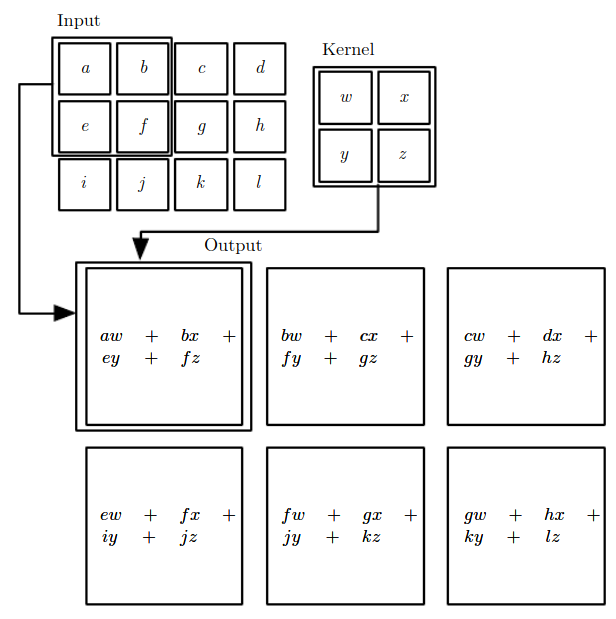
\includegraphics[width=0.6\textwidth]{imagens/ilustracoes/cap2_convolucao.png}
  \par \textbf{Source: \citeonline{{Goodfellow2016}}}
  \label{fig:cap2_convolucao}
\end{figure}

After a convolutional filter, a two-dimensional activation map is produced.
Multiple activation maps are stacked into an adjacent layer.
The network uses these maps in the following layers, in order to produce different features.
These features can be grouped together to produce predictions \cite{Albawi:2017} \cite{OShea:2015}.

%-----------------------------------------------
%SUB - OPERAÇÃO CONVOLUÇÃO
\subsection{Transposed Convolution Operation}
\label{cap2_deconvolucao}

The transposed convolution operation stems from the need to use an operation contrary to the traditional convolution.
It is also called deconvolution, although transposed convolution is not necessarily the reverse of convolution operation.
The operation allows the retrieval of an initial features map that has undergone a convolution process. \cite{Dumoulin:2016}.

The transposed convolution can be emulated using a traditional convolution.
This requires rebuilding a processing space.
The solution is to create borders with zero values around the image and also between pixels, in the minimum amount required.
Then the convolution is applied over the constructed space \cite{Dumoulin:2016}.

%-----------------------------------------------
%SUB - POOLING
\subsection{Pooling Operation}
\label{cap2_pooling}

The pooling function, commonly used in convolutional networks, is used to provide statistical information about nearby outputs.
It aims to maximize the advantages of the output and become invariant to small noises or translations.
Pooling functions can also be used to reduce the amount of neurons between network layers by grouping results into the next layer. 
Among the existing functions, the max-pooling operation highlights, which gets the maximum value from a set of outputs \cite[Ch. 9]{Goodfellow2016}.
